%%%%%%%%%%%%%%%%%%%%%%%%%%%%%%%%%%%%%%%%%%%%%%%%%%%%%%%%%%%%%%%%%%%%%%%%%%%%%%%

\chapter{Einleitung}
Dieser Praxisbericht thematisiert das Messen von Schiffsemissionen durch den Emissionsmesser MARSIC300, der SICK AG. Dabei wird der technische Rahmen um die Entstehung und Filterung von Schiffsemissionen erläutert woraufhin beschrieben wird weshalb, die Messung von Schiffsemissionen zwingend erforderlich ist im Hinblick auf regulatorische und rechtliche Aspekte. Auch soll ein genauerer Einblick in die Funktionsweise des MARSIC300 gegeben werden, so wie auch die Kozeptionierung von Anwendungsmöglichkeiten im Bezug auf Servicedienstleistungen durch die Analyse von gesammelter Big Data, mit der Hilfe von marinetraffic.com. Die Ergebnisse werden darauf hin evaluiert und ein Ausblick zur zukünftigen Weiterentwicklung wird gegeben. Diese Praxisarbeit dient unter anderem zur theoretischen Vorbereitung auf die Bachelorarbeit. 
%%%%%%%%%%%%%%%%%%%%%%%%%%%%%%%%%%%%%%%%%%%%%%%%%%%%%%%%%%%%%%%%%%%%%%%%%%%%%%%

\section{Projektumfeld}

%%%%%%%%%%%%%%%%%%%%%%%%%%%%%%%%%%%%%%%%%%%%%%%%%%%%%%%%%%%%%%%%%%%%%%%%%%%%%%%

\subsection{Firma}
Das Unternehmen Sick AG wurde 1946 von Erwin Sick gegründet und zählt mit einer Vielzahl von Sensorlösungen vor allem in der Fabrik-, Logistik- und Prozessautomation zum Markt- und Technologieführer für Sensorintelligenz. Die Sick AG ist global in über 80 Ländern mit 50 Tochtergesellschaften vertreten und beschäftigt weltweit über 10.000 Mitarbeiter. Dabei wächst das Unternehmen stetig und erwirtschaftete beispielweise im Geschäftsjahr 2019 einen Umsatz von rund 1,8 Mrd. Euro\cite{SICK.2021a}.
\begin{figure}[H]
\centering
\fbox{\includegraphics[height=0.15\textheight]{Bilder/SickFirmenGebäude}}
\caption{\label{fig-firmenHQ}Der Firmen Sitz der Sick AG in Waldkirch}
\end{figure}
%%%%%%%%%%%%%%%%%%%%%%%%%%%%%%%%%%%%%%%%%%%%%%%%%%%%%%%%%%%%%%%%%%%%%%%%%%%%%%%
\subsection{Abteilung}
Das Global Industrie Center Process Automation unterteilt sich in 5 Untersegmente mit den Schwerpunkten Basic Materials, Infrastructure, Oil and Gas, International Tender Management und Area sales support. Die teilweise wiederum Unterteilt werden können. 
Das Projekt findet dabei in der Abteilung mit dem Schwerpunkt Comubustion enginnes/Maritime unter der Leitung von Hinrich Brumm statt. Primäre Aufgabe der Gruppe ist es effiziente Lösungen für Industrien mit dem Schwerpunkt auf Verbrennung Prozessen zu finden. Beispiele wäre dabei eben die Verbrennung von Diesel. 
%%%%%%%%%%%%%%%%%%%%%%%%%%%%%%%%%%%%%%%%%%%%%%%%%%%%%%%%%%%%%%%%%%%%%%%%%%%%%%%

\section{Motivation}
Mit einem jährlichen Umsatz von bis zu 1 Mrd. Tonnen CO$_{2}$ ist die Schifffahrt für etwa 3\% der Weltweiten Emission verantwortlich. Damit ist sie auf gleicher Höhe mit der Luftfahrt und ca. 5 mal kleiner als der durch den Straßenverkehr verursachten CO$_{2}$ Emissionsanteil Weltweit(vgl. \cite[S. 584]{EnergyPolicy.2016a}).
\begin{figure}[H]
\centering
\fbox{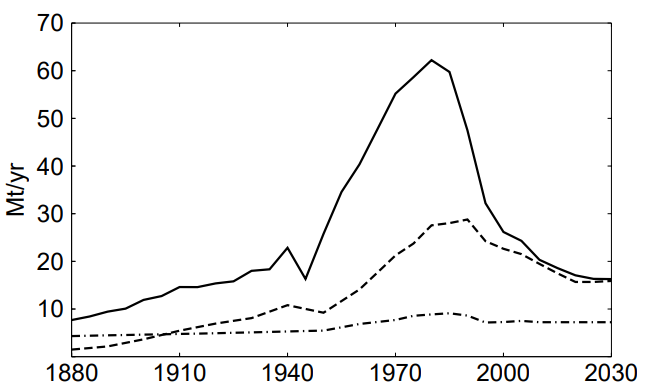
\includegraphics[height=0.3\textheight]{Bilder/DiagrammSchwefel}}
\caption{\label{fig-firmenHQ}Zeitliche Entwicklung der Europäischen Emission von SO$_{2}$(durchgängig), NO$_{x}$(gestrichelt) und NO$_{3}$}
\end{figure}
Während jedoch der Trend des NO$_{x}$ und SO$_{2}$ Emissionsgehalt seit den 1980ern laut Wissenschaftsjournal \textit{Hydrology \& Earth System Sciences} sinkt\cite{HandE.2003a}, ist die Schifffahrt deutlich verantwortlicher für den Schadstoffausstoß und sorgt mit dafür, dass der Trend langsam aber sicher abflacht und stagniert. So beträgt der Beitrag für NO$_{x}$ und SO$_{2}$ durch Schiffsemission 15\% und 13\%, Entwicklung steigend.\\Mit unter Grund für die Drosslung des SO$_{2}$ Gehalts in den letzten 30 Jahren ist die Einführung von Normen für Kraftfahrzeug Kraftstoff auf der ganzen Welt. So ist es beispielsweise nur gestattet, laut der seit 2005 geltenden EURO IV Norm, Treibstoff zu Tanken mit einem Schwefelgehalt von 50pm\cite{Kfz_Auskunft}. Länder wie beispielsweise Deutschland fördern durch steuerliche Bonitäten die Einfuhr von schwefelfreien Kraftstoff mit einem Schwefel gehalt von 10ppm was 0,001\% entspricht\cite{Zoll}. Im maritimen Sektor hingegen waren bis vor 2020 Treibstoff mit einem Schwefelgehalt von maximal 3.5\% erlaubt was seit 2020 durch die International Maritime Organization(IMO)auf 0.5\% Weltweit gesengt wurde.
\\
Erdöl oder auch Rohöl enthält je nach Herkunft unterschiedliche Konzentrationen an organischen Schwefelverbindungen. Um niedrige bzw. normgerechte Schwefelanteile zu erhalten muss das Öl entschwefelt werden, was Kosten verursacht und dem Entsprechend den Preis steigert. Gerade bei Schiffen, die mit ihrem großen Gewicht enorme Distanzen zurück legen müssen, ist der Verbraucht sehr Hoch. So kann ein Containerschiff um die. 200 Litern pro Seetag verbrauchen, weshalb die Reedereien daran interessiert so billig wie möglich zu tanken. Dabei bleibt den Reedereien zwei Möglichkeiten um auf gesetzte zu reagiert:
\begin{enumerate}
\item Treibstoff tanken mit entsprechendem Schwefelgehalt.
\item Den Schwefel und auch andere Schadstoffe aus der Emission zu filtern.
\end{enumerate}
Punkt 2. lässt sich dabei durch technische Filtermechanismen realisieren. Damit das Schiff verifizieren kann, dass die gefilterten Emissionen allen Auflagen entsprechen müssen die Abgase kontinuierlich analysiert werden. Der MARSIC300 realisiert dabei diese Aufgabe.        
%%%%%%%%%%%%%%%%%%%%%%%%%%%%%%%%%%%%%%%%%%%%%%%%%%%%%%%%%%%%%%%%%%%%%%%%%%%%%%%

